%
\documentclass{acmtog}
\usepackage{indentfirst}
\usepackage[utf8]{inputenc}
\usepackage{amsmath}
\usepackage[retainorgcmds]{IEEEtrantools} %IEEEeqnarray
\usepackage{listings}
\usepackage{hyperref}

\lstset{
    language=C,
    tabsize=2,
    breakatwhitespace=false,
    basicstyle=\ttfamily\footnotesize\bfseries,
    captionpos=b,
}

\renewcommand*{\lstlistingname}{Listing}

\acmVolume{VV}
\acmNumber{N}
\acmYear{YYYY}
\acmMonth{Month}
\acmArticleNum{XXX}  
\acmdoi{10.1145/XXXXXXX.YYYYYYY}

\acmVolume{}
\acmNumber{}
\acmYear{2012}
\acmMonth{02}
\acmArticleNum{}
\acmdoi{}

\begin{document}

\markboth{Miguel Palhas}{Overview of Lindenmayer Systems}

\title{Overview of Lindenmayer Systems} % title

\author{Miguel Palhas
\affil{Universidade do Minho}}

\category{F.4.2}{Grammars and Other Rewriting Systems}{L Systems}
\category{I.3.5}{Computer Graphics}{Computational Geometry and Object Modeling}[Physically based modeling]
\category{I.3.5}{Computer Graphics}{Computational Geometry and Object Modeling}[Object hierarchies]
\category{I.3.7}{Computer Graphics}{Three-Dimensional Graphics and Realism}[Animation]
\category{I.3.7}{Computer Graphics}{Three-Dimensional Graphics and Realism}[Fractals]

%\terms{Experimentation, Human Factors}

%\keywords{Face animation, image-based modelling, iris animation, photorealism, physiologically-based modelling}

%\acmformat{Pamplona, V. F., Oliveira, M. M., and Baranoski, G. V. G. 2009. Photorealistic models for pupil light
%reflex and iridal pattern deformation.  {ACM Trans. Graph.} 28, 4, Article 106 (August 2009), 11 pages.\newline  DOI $=$
%10.1145/1559755.1559763\newline http://doi.acm.org/10.1145/1559755.1559763}

\maketitle

%\begin{bottomstuff} 
%Manuel M. Oliveira acknowledges a CNPq-Brazil fellowship (305613/2007-3). Gladimir V. G. Baranoski acknowledges a
%NSERC-Canada grant (238337). Microsoft Brazil provided additional support.
%
%Authors' addresses: land and/or email addresses.
%\end{bottomstuff}

\begin{abstract}
A look into L-Systems, a formal method of defining structures that exhibit recursive or self-similar patterns. Some recent platforms that use L-Systems are referenced, for their contribution to the field, and it's possible usefulness in either scientific analysis, or real time applications, like games or simulators. An overview is given on some potential applications of L-Systems, such as biology or architecture, and also some of the supporting platforms and languages that can be used to achieve this.
\end{abstract}


%%%%%%%%%%%%%%%%%%%%%%%%%%%%%%%%%%%%%%%%%%%%%%%%
%%%%%%%%%%%%%%%%%%%%%%%%%%%%%%%%%%%%%%%%%%%%%%%%
\section{Origin}
\label{sec:origin}

L-Systems were introduced in 1968 by a Hungarian biologist, Aristid Lindenmayer. Lindenmayer studied the patterns that can be observed in the growth of several types of plants. The original idea was to provide a formal method of describing the development of simple organisms. Later on, they started to be used to for more complex structures.



%end sec{origin}

%%%%%%%%%%%%%%%%%%%%%%%%%%%%%%%%%%%%%%%%%%%%%%%%
%%%%%%%%%%%%%%%%%%%%%%%%%%%%%%%%%%%%%%%%%%%%%%%%
\section{Basic Structure and Properties}
\label{sec:basicstruct}

A Lindenmayer system (more commonly known simply as L-system) is a type of rewriting system, a general tool for constructing complex objects by starting with a simple object and recursively replacing parts according to instructions provided by a set of rewriting rules.

Formally, an L-System is a grammatical method to proceduraly model a system. It is generically represented as:

\begin{equation}
  G = (V, \omega , P)
  \label{eq:genericsystem}
\end{equation}

where:
\begin{description}
  \item[\textbf{V}] is the alphabet, a set of symbols defining the elements that compose the language of system we are describing. These symbols can be concatenated into strings;
  \item[\textbf{$\omega$}] is the axiom, or the initial string upon which the system will operate to generate the final geometry;
  \item[\textbf{P}] is the set of production rules, that define how the strings are replaced to form new combinations.
\end{description}

It's also necessary to provide a depth level ($n$), to indicate how deeply the productions should be processed, to control the level of detail of the final geometry.

These are the components of a regular grammar, from which L-Systems are derived. Aside from those attributes, the system must also define a translation mechanism which maps each of the resulting strings into a geometric structure, in order to generate the final result.

The system works by applying the rules iteratively to a string, whose initial value is given by w. As oposed to a conventional formal grammar, which applies a single rule at a time, in this case many rules can be applied simultaneously in a single iteration.

If each production refers only to an individual symbol and to its neighbours, the system is considered to be context-free. This subset of L-Systems are specified by a regular grammar. If the rules depend also on the neighbour symbols, then it is a context-sensitive L-System.

An L-System can also be non-deterministic or deterministic. If only one rule can apply to each symbol, then it is deterministic, as the final result will not change as long as neither of the initial parameters also remain the same. However, there may be several rules applying to the same symbols, and a defined method of selecting between each one. If this method is probabilistic, then the system is a stochastic L-System.

%end sec{basic structure and properties}

%%%%%%%%%%%%%%%%%%%%%%%%%%%%%%%%%%%%%%%%%%%%%%%%
%%%%%%%%%%%%%%%%%%%%%%%%%%%%%%%%%%%%%%%%%%%%%%%%
\section{Example}
\label{sec:example}

shows the original example showed by Lindenmayer, which models the growth of algae:
\begin{eqnarray*}
  V   &=& \{A, B\}           \\
  \omega       &=& A                   \\
  P       &=& \{A \rightarrow AB,   \\
              & & B \rightarrow A \}  
  \label{eq:example1}
\end{eqnarray*}


this system produces the following result on the first iterations:

\begin{IEEEeqnarray*}{l}
  n=0: A  \\
  n=1: AB \\
  n=2: ABA  \\
  n=3: ABAAB  \\
  n=4: ABAABABA 
\end{IEEEeqnarray*}

The recursive nature of the system can be seen in this example, as the resultant string becomes larger with every iteration

%%%%%%%%%%%%%%%%%%%%%%%%%%%%%%%%%%%%%%%%%%%%%%%%
%%%%%%%%%%%%%%%%%%%%%%%%%%%%%%%%%%%%%%%%%%%%%%%%
\section{Rendering}
\label{sec:rendering}

After defining the grammar for the desired model, a method is required to generate a graphical imagem based on the symbols acquired from iterating through the grammar. A common method to perform this is with Turtle graphics.

Turtle graphics is a computer graphics technique used for vector graphics that works a state machine using a cursor (also called the "turtle") in a Cartesian Plane. In this method, commands are given to alter the state of the turtle, which has simple properties like position, orientation, color, or drawing state. When the drawing state is true, the turtle acts like a pen, drawing as it moves. The turtle can receive commands such as "\textit{move forward 5 units}" or "\textit{turn left by 30 degrees}", effectively altering the current state.

From this basic building blocks, more complex algorithms can be made. Consider the following function that instructs the turtle to draw a simple square:

\begin{lstlisting}[label={lst:square}]
  draw_box() {
    forward(10);
    turn(90);
    forward(10);
    turn(90);
    forward(10);
    turn(90);
    forward(10);
    turn(90); 
  }
\end{lstlisting}

This function can then be used to draw even more complex shapes, such as a group of boxes:

\begin{lstlisting}[caption={},label={lst:squares}]
  draw_boxes() {
    draw_box();
    turn(90);
    draw_box();
    turn(90);
    draw_box();
    turn(90);
    draw_box();
    turn(90);
  }
\end{lstlisting}

\autoref{fig:boxes} illustrates the result of both this functions.

\begin{figure}[!htp]
  \begin{center}
    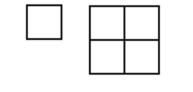
\includegraphics{images/0_draw_box}
    \caption{Squares drawn with turtle graphics \label{fig:boxes}}
    \end{center}
\end{figure}

Of course, the amount of instructions that can be issued to the turtle is implementation-dependant, and can be much more complex as just moving forward and rotating. Concepts like memory, stacks, probabilities and functions can be implemented to further increase the capabilities of the turtle.

%%%%%%%%%%%%%%%%%%%%%%%%%%%%%%%%%%%%%%%%%%%%%%%%
%%%%%%%%%%%%%%%%%%%%%%%%%%%%%%%%%%%%%%%%%%%%%%%%
\section{Pairing L-Systems with Turtle Graphics}
\label{sec:pairing}

In an L-System, strings are recursively expanded into other strings based on the set of production. If we interpret each Symbol of a string as a turtle command, then we can look at the whole string given by the L-System as a whole function that can be issued to render turtle geometry..

Let's assume the following symbols, and their corresponding turtle command:

\begin{eqnarray*}
    F & \rightarrow &  forward()  \\
    + & \rightarrow &  turn(\alpha)   \\
    - & \rightarrow &  turn(\alpha)  
\end{eqnarray*}

And also, the following L-System:

\begin{eqnarray*}
  \alpha  &=& 60                         \\
  V       &=& \{F, -, +\}                \\
  \omega  &=& F--F--F                     \\
  P       &=& \{F \rightarrow F+F--F+F \}    
\end{eqnarray*}

Without applying any productions ($n=0$), $\omega$ is unchanged, and according the previously defined turtle commands, the rendered result will be:

\begin{figure}[!htp]
  \begin{center}
    
\includegraphics{images/1_triangle}
    \caption{Triangle drawn with Turtle Graphics \label{fig:triangle}}
    \end{center}
\end{figure}

With $n=1$ the production is applied once, which means that all $F$ Symbols in $\omega$ will be expanded. As $n$ increases, so does the complexity of the result. \autoref{fig:triangle_detail} shows the increasing detailed results of this L-System for $1 \leq n \leq 4$

\begin{figure}[!htp]
  \begin{center}
    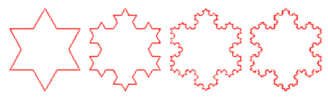
\includegraphics{images/2_triangle_detail}
    \caption{Expansion of the Triangle L-System \label{fig:triangle_detail}}
    \end{center}
\end{figure}

This is actually an example of a widely popular L-System, known as the Koch Snowflake, due to it's resemblance to a snowflake as the image gets more detailed.

%%%%%%%%%%%%%%%%%%%%%%%%%%%%%%%%%%%%%%%%%%%%%%%%
%%%%%%%%%%%%%%%%%%%%%%%%%%%%%%%%%%%%%%%%%%%%%%%%
\section{Functionality}
\label{sec:functionality}

\subsection{Branching}
\label{subsec:branching}

Let's now add some more operator to the symbol list:

\begin{eqnarray*}
    [ & \rightarrow &  push_state() \\
    ] & \rightarrow &  pop_state() 
\end{eqnarray*}

Where push\_state() is a function instruct the turtle system to store it's current state in a stack, and pop\_state() instructs it to reload the last saved state, removing it from the stack. With the introduction of a stack, the turtle can effectively recover previous states, allowing for branched geometries to be rendered, continued from a previous point of the geometry that is not the most recently drawn. For instance, consider now the following L-System and its corresponding result for different $n$ values:

\begin{eqnarray*}
  \alpha  &=& 30                         \\
  V       &=& \{F, -, +, [,\; ]\}        \\
  \omega  &=& F                           \\
  P       &=& \{F \rightarrow F[-F]F[+F]F\} 
%  \label{eq:example2}
\end{eqnarray*}

\begin{figure}[!htp]
  \begin{center}
    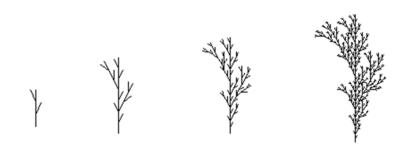
\includegraphics[width=\columnwidth]{images/3_tree}
    \caption{Trees drawn with Turtle Graphics \label{fig:tree}}
    \end{center}
\end{figure}

The stack operator can be useful to allow the turtle to explicity recover previous states, allowing complex geomtries that resemble weeds and other types of vegetation.

\subsection{Parametric L-Systems}
\label{subsec:parametric}

An L-System can support parameters which can be useful to use the same system to generate geometries with a certain degree of variety. For example, a generator for a tree leaf can be parameterized with the leaf's color and length, resulting in the creation of several different leafs which, even though are sharing a common structure, have some noticeable differentes between them.

Another useful capability of parameters is to allow the same productions to be used to achieve different results, according to the parameters that are give to them. The preivous example to render weeds can be extended with parameters to add some variety to the result.

A parametric L-System can also include conditional productions, so that they are only applied when their parameters meet a condition, as shown in the following example:

\begin{eqnarray*}
  V       &=& \{F\}                                               \\
  \omega  &=& F(4,4)                                              \\
  P       &=& \{                                                  \\
          & & F(x,y) : x \leq 3 \rightarrow F(x \times 2, x + y,  \\
          & & \, F(x,y) : x >    3 \rightarrow F(x / y, 0\        \\
          & & \}                                                  
  \label{eq:example3}
\end{eqnarray*}

\subsection{Stochastic L-Systems}
\label{subsec:stochastic}

An L-System can also be parameterized with probabilistical values, allowing for a somewhat random effect to be added, creating more diverse and natural results. This is called a Stochastic L-System. Consider the following example:

\begin{eqnarray*}
  V       &=& \{F, -, +\}                   \\
  \omega  &=& F                             \\
  P       &=& \{                            \\
          & & F : (0.5) \rightarrow [+FF]F, \\
          & & F : (0.5) \rightarrow [-FF]F, \\
          & & \}                            
  \label{eq:example4}
\end{eqnarray*}

In this system, when expanding the $F$ symbol, both productions might be used. However, unlike in the example shown in \autoref{subsec:parametric}, where the choice was determined by the parameters given to the system, here, the choice is probabilistical. There is a $50\%$ change for each production to be used each time. In this example, one production creates a branch on the right side of the structure, while the other does the same on the left side. So at each step, a branch will be created on a randomly chosen side. \autoref{fig:stochastic} shows four different results achieved using this L-System.

\begin{figure}[!htp]
  \begin{center}
    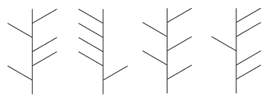
\includegraphics[width=0.6\columnwidth]{images/4_stochastic}
    \caption{Stochastic L-System structures \label{fig:stochastic}}
    \end{center}
\end{figure}

\subsection{Context Sensitive L-Systems}
\label{subsec:context}

Like a regular L-System follows the usual rules of a regular grammar, a context-sensitive L-System is one based on context-sensitive grammars, trying to match both sides of a symbol when applying a production. With a context-sensitive l-system, the application of a production depends not only on the symbol in which it is being applied, but also on it's predecessor and successor. A possible representation of a production for this kind of systems is:

\begin{eqnarray*}
  a_{l} < a > a_{r} : \chi \\
\end{eqnarray*}

meaning that for a given symbol $a$, a substitution by the word $\chi$ will occur if $a$ is preceded by $a_{l}$ and succeeded by $a_{r}$.


\subsection{Self-sensitive L-Systems}
\label{subsec:selfsensitive}

All functionality described so far does not take into account that in an L-System, different branches of a structure might be influenced by other branches, and ultimately may result in the merging of these branches. This is not so commonly used, but is still a topic of interest in the generation of some structures that required a closed-circuit topology.

The main difficulty with this systems is because, since the productions are applied recursively for each depth level, when processing one level, the current state of the system can only have knowledge of the previously calculated depth level, while in some cases it could be required that an iteration can be influenced by other branches in a more advanced state. This holds true for systems where the growth is not uniform, as is the expansion of productions in the L-System that represents it.

\subsection{Interaction-sensitive L-Systems}
\label{subsec:interactionsensitive}

Just like self-sensitive L-Systems, dealing with external interactions also poses a difficult problem. Some systems, in order to create useful representations, require that exterior factors can influence the object growth. These factors have a wide variety, such as environmental factors (properties of the environment in which the system is growing), user input (for interactive systems that change with time) or even other L-Systems growing in parallel.

%%%%%%%%%%%%%%%%%%%%%%%%%%%%%%%%%%%%%%%%%%%%%%%%
%%%%%%%%%%%%%%%%%%%%%%%%%%%%%%%%%%%%%%%%%%%%%%%%
\section{Fractals}
\label{sec:fractals}

A fractal is an object that displays a self similar pattern at all scales. This means that zooming in on a finite portion of the object shows similar properties to the whole object, and this recursion is preserved infinitely.

\begin{figure}[!htp]
  \begin{center}
    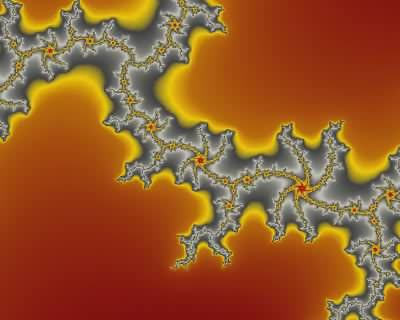
\includegraphics[width=0.8\columnwidth]{images/5_1_fractal}
    
\includegraphics[width=0.8\columnwidth]{images/5_2_fractal}
    \caption{Fractal images \label{fig:fractais}}
    \end{center}
\end{figure}

Because of this self similarity properties, a fractal can usually be described with an L-System. The Koch snowflake, already shown in \autoref{sec:pairing} is a known example of a fractal image generated by an L-System. Another example is the Sierpinski Triangle \cite{FRACTALS}, which can actually be implemented in more than one way. One of the possible implementations is as follows:

\begin{eqnarray*}
  \alpha  &=& 60                        \\
  V       &=& \{F, G, -, +\}            \\
  \omega  &=& F                         \\
  P       &=& \{                        \\
          & & F \rightarrow G-F-G,      \\
          & & G \rightarrow F+G+F       \\
          & & \}                        
\end{eqnarray*}

\begin{figure}[!htp]
  \begin{center}
    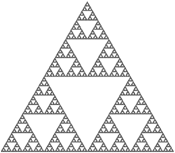
\includegraphics[width=0.8\columnwidth]{images/6_sierpinski}
    \caption{Fractal images \label{fig:Sierpinski Triangle}}
    \end{center}
\end{figure}

The method used here uses two symbols, $F$ and $G$ to declare movement. For the turtle implementation, both of these symbols provide the same result, which is to move forward drawing a line. However, their difference is in choice of the productions to use. Since each of them have a different production associated with them, they are threated separately and replaced with a different string when the result is being expanded.

%%%%%%%%%%%%%%%%%%%%%%%%%%%%%%%%%%%%%%%%%%%%%%%%
%%%%%%%%%%%%%%%%%%%%%%%%%%%%%%%%%%%%%%%%%%%%%%%%
\section{L-Systems and Programming}
\label{sec:languages}

There are already a few attempts of implementations of programming languages with a focus on L-System declaration

\subsection{The L+C Modeling Language}
\label{subsec:lc_language}

The L+C Language \cite{karwowski2003design} is a C++ based language that combines a L-System constructs with the general-purpose language C++. The constructs have a syntax that is similar in many ways to traditional L-System notation.

A typical L+C program has the following structure:

\begin{lstlisting}[label={lst:lc_example}]
  #include <lpgfall.h>
  // declarations of data structures
  // declarations of functions
  // declarations of modules
  derivation length: n;
  axiom: module_list;
  // productions;
\end{lstlisting}

\emph{lpfgall.h} is the standard library for \emph{lpfg} files (a plant modeling program to render L+C code). It includes some standard C/C++ libraries required for the program, and also defines some default structures and parameters used throughout the program.

\subsubsection{L+C Constructs}
\label{subsubsec:constructs}

An L+C program can be divided into C++ declarations and L-System constructs. These constructs are declarations like the \emph{derivation length: n} shown in the example, and are processed by the L2C, or L+C to C converter, before compilation. The derivation length defines how many steps the execution should be take, or in other words, the depth of the final result. A bigger length will result in finer, more detailed results, but with the increased execution time.

The constructs also include

\subsection{L-Studio}
\label{subsec:lstudio}

L-studio is a simulation software used to create visual simulations of models using L-Systems \cite{LSTUDIO}.
It's core functionality is in the two simulation programs: \emph{cpfg} and \emph{lpfg}. These programs receive an L-System as input and use it to produce a visual representation of the provived model. The models described may be animated and/or allow for interaction. Some output data may also be provided during the simulation. While \emph{cpfg} and \emph{lpfg} both share a common interface, the first is suitable for rapid creation of simple models, while the second is more useful when attempting more complex simulations.

%%%%%%%%%%%%%%%%%%%%%%%%%%%%%%%%%%%%%%%%%%%%%%%%
%%%%%%%%%%%%%%%%%%%%%%%%%%%%%%%%%%%%%%%%%%%%%%%%
\section{Applications}
\label{sec:applications}



L-Systems have been proven useful since their first appearance by Lindenmayer to be useful for the modeling of plants and other organic organisms. Lindenmayer himself, as a biologist, started to develop this mechanism to represent the various patterns that were noticeable in multicellular organisms. This was later extended to the representation of bigger organisms, such as plants, and other complex branching structures with self similarity properties.

\subsection{Plant Modeling}
\label{subsec:plant_modeling}

Plant modeling and virtual visualization can be applied for a variety of purposes \cite{hanan1992parametric}. In biology, a virtual representation of a plant can be useful to study mechanisms associated for example, with the flowering of that plant. A research may conceptualize a model based on previous research and observation, gather data which is deemed important, and build a model that represents the already known information about the organism. Later, with the visualization of the built model, inaccuracies can be revealed, which might indicate errors or invalid assumptions in the model, or maybe overlooked factors that contribute to the state of the model, and are preventing it from behaving like the real-life version of it.

Using a parameterized L-System to represent these models will also allow them to be better tuned, and find approximations of the parameters that make the model reach resemblance to real-life samples.

When a built model is considered valid, it can be used in many areas. An analysis of the model can help in the understanding of the development mechanism and their effect on plant morphology. It can also allow the study of evolutionary trends in plant architecture, and even to provide predictions for real-life samples.

For example, plant models have been used for some time to study the transport of light in vegetative canopies. Ecology is also an area of interest, where the models can be used to study the interaction between plants and their environments.

Animations are also an important part of plant modeling, as they provide a way to visualize plant growth, which in turn is helpful to clarify some properties of this process.

\subsection{Interactions}
\label{subsec:interactions}

The interactions between a plant and it's environment has also been a field of study that has benefited from the use of L-Systems. Both the plant and the environment require a detailed representation, which is usually difficult to formulate and implement. Previous applications designed to assist in this simulations lacked some important characteristics. Some of them that were directed towards the scientific community would limit the simulation to a small group of plants of a certain family, and the rendered results would have a rudimentary graphical design. Others relied more on finely detailed models, and were designed with a emphasis on the graphical detail, but in turn lacked the functionality to faithfully reproduce the mechanisms and characteristics that were inherent to the plant itself.

Therefore arose the need for a common framework, that could provide accurate results, not only at the rendering and detailing of the objects visualization, but also at the calculation of it's interactions with other plants and the environment.

As described in \cite{mech1996visual}, there is already some work towards a tool for the simulation of interactions and their effect on L-Systems. While this particular solution was designed to work with plant interactions, the concepts can also be applied to a wide range of fields where the relations between different elements need to be modeled.

\begin{figure}[!htp]
  \begin{center}
    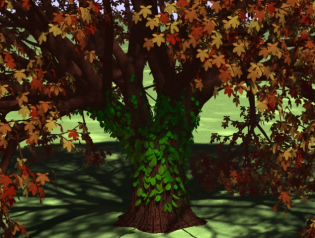
\includegraphics[width=0.8\columnwidth]{images/7_plants}
    \caption{Rendering of a climbing plant growing on a tree \label{fig:relations}}
    \end{center}
\end{figure}


\begin{figure}[!htp]
  \begin{center}
    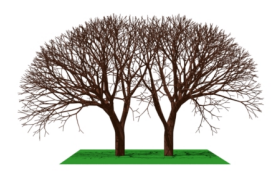
\includegraphics[width=0.8\columnwidth]{images/8_plants}
    \caption{Two trees competing for light \label{fig:relations_2}}
    \end{center}
\end{figure}

When attempting to simulate interactions, there are a lot of factors that should be taken into account. For instance, the proposed implementation deals with problems such as:
\begin{description}
  \item[Root development] The roots of any plant cannot be modeled independently, as their growth strongly depends on the characteristics of the environment.
  \item[Light sources] Since plants tend to growth towards the sunlight, when considering large groups of plants, it should be expected that they will compete for the light, sometimes blocking each other, thus affecting each other's growth pattern.
  \item[Limited space] When dealing with a large number of growing objects, space can also become a relevant factor, as trees become larger, and start competing with others, not only for resources, but also for space. As a result, their structures might collide at some point, or event cooperate with each other.
\end{description}

\subsection{Real Time Tree Generation}
\label{subsec:realtimetrees}

In computer graphics, trees and other types of vegetation are often a challenge. While hand made models can have a good visual result, this approach would lack the variety required between multiple instances of a tree, lowering the overall quality of a large scale scene. As already shown in previous sections, trees exhibit a self-similar geometry, and can be modeled precisely using L-Systems.
However, unlike pure fractal objects, a tree is not strictly auto-similar. Some randomness is also applied during the generation, to allow for diversity between the different elements of a tree. This can be considered statistically self-similar geometry.

This statistical properties introduce additional information, and also an increased number of calculations necessary to generate the geometry. Therefore, a compromise must be made in order to achieve real-time usable results. \cite{baele2005real} proposes a hybrid CPU/GPU approach with L-Systems and Turtle Graphics.

The solution attempts to balance the work load between the CPU and the GPU, while also minimizing data transfers between the two. An initial generation of the L-System is done on the CPU. It relies on SSE instructions to efficiently calculate the appropriate turtle command for a given symbol, which mostly translates to a matrix transformation operation. After this step, the rendering of each branch is split between the first phase, where data is sent to the graphics board and the second phase, all the vertices are processed.

As a tree can be though of as static after it has been generated once, the cost of sending data to the GPU can be minimized, by reutilization of the previous values. This way, only positioning matrices are required for every new calculation.

Since computational performance is required to allow for real time rendering, there had to be a compromise with the detail of the result. Because of this, the solution performs the rendering of the tree using different levels of detail for each degree of visibility. One example of this compromise is with the processing of leaves. Even though they are lighter in terms of vertex processing, since they are positioned in a higher position of the tree hierarchy, they appear in greater number, and create a problem for the CPU processing phase, by generating a lot of turtle instructions.
One possible solution to decrease the computational weight is to use impostors, which is a widely used method for the rendering of trees, to allow for fast rendering when the object is far away in the scene.

As for lighting, the solution considers that lighting is more important on the leaves, when the observer is far from the tree and it can be considered one single object, but as the distance decreases, more processing must be made on the lighting of branches. For the leaves, lighting is calculated based on the leaf's relative position to the tree, making it so that leaves that are on the outer region of the tree have a bigger illumination factor that interior leaves. Branches are more difficult to calculate, as the fractal geometry of a tree is not suitable for the calculation of a shadow volume. Instead, a generic shadow map is used for each different combination of L-System and its parameters. The result, while not theoretically correct, is good enough for real time rendering.

Note that at the time of development of the solution, graphics cards were starting to achieve the required performance to enable this kind of rendering. All tests shown on \cite{baele2005real} were performed using a system that is considered outdated by today's standards (Pentium 4 1.5GHz, GeForce FX 5900). More recent graphics cards should allow for a significant increase in either computational time, or level of detail in the final geometry.

\begin{figure}[!htp]
  \begin{center}
    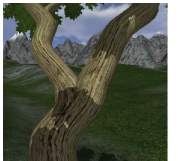
\includegraphics[width=0.6\columnwidth]{images/11_realtime}
    \caption{Shadow on a generated tree \label{fig:realtime2}}
    \end{center}
\end{figure}

\subsection{Computational Architecture}
\label{subsec:architecture}

Just as natural organisms exhibit self-similarity properties which allow them to be represented by an L-System, this can also hold true when talking about artificial structures. In the case of plants, it can be simply said that each plant is composed of branches, with a somewhat regular pattern (not entirely predictable, but still following some basic properties that are inherent to the object itself), which in turn end in flowers, or other elements. Going even further, an L-System can be created based on those plants, to create a larger group, where some rules about their distribution can be applied. For example, some plants may favor places where other plants of a certain species exist, they may grow in groups or individually.

This concepts can be translated to other large scale, and possibly not natural elements. Cities for example, exhibit similar properties. A city can be though of as a collection of buildings, that follow a certain distribution pattern (usually bigger and more concentrated in the center of the city), and are surrounded by other elements, such as streets, parks, or any other object. Each building can then be modeled individually, as the same logic applies to them.

An L-System based approach called \emph{CityEngine} has been developed with capabilities to model a complete city using a small set of input data, such as information on the geography of the terrain, or statistical information about population concentration. This is an example of where a self-sensitive L-System implementation can be useful. The streets in a city can branch themselves with fractal-like properties, but they also form a closed system. A regular L-System approach cannot be used to model this behavior, as it does not provide the capability of representing a self-sensitive system.

In order to achieve a self-sensitive result, the approach was to, after generating a segment of a street, checking it for collisions with other existing segments. In the event a collision, the road is pruned, generating a crossing. \autoref{fig:pruning} shows the behavior used.

\begin{figure}[!htp]
  \begin{center}
    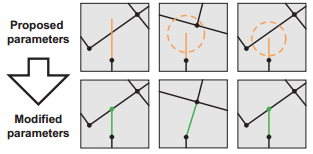
\includegraphics[width=0.7\columnwidth]{images/12_selfsensitive}
    \caption{Self-sensitive street generation of a city \label{fig:pruning}}
    \end{center}
\end{figure}

\autoref{fig:cities} shows the pipeline for the proposed solution.

\begin{figure}[!htp]
  \begin{center}
    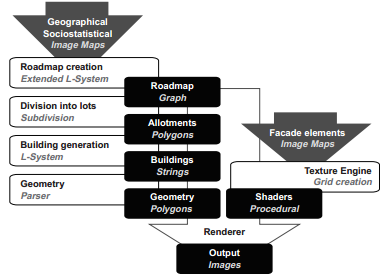
\includegraphics[width=0.8\columnwidth]{images/9_cities}
    \caption{Pipeline for the city creation tool \emph{CityEngine}. Dark boxes show results and data of the individual tools, shown in white \label{fig:cities}}
    \end{center}
\end{figure}

The tool works by first feeding the input to a road-generation system. This system uses an approach where streets are categorized in two main classes: main streets and side-roads. While main streets usually exhibit a radial behavior, with multiple streets converging around a centric point, side-roads have a raster oriented pattern. Based on this, the road generation uses some patterns to apply in different scenarios, allowing for different zones of the city to follow different rules.

After the generation of the streets, a new subdivision is made, dividing the city into blocks, each block will consist of multiple buildings. These buildings, in turn, can be generated with a parametric, stochastic L-System. A lot of factors can come into play here, like the usage of higher buildings only in blocks located in the center of the town, or event regulations about the size of the buildings for a given city zone.

Textures are then applied to the scene, based on actual pictures of buildings, which are modified and projected onto each surface. Procedural textures can also be used to reduce the amount of work to prepare the textures for each building.

The final result is a system that is capable of generating a large-scale city based on a small size, two dimensional input, mostly with the usage of parametric and stochastic L-Systems to generate high fidelity results. \autoref{fig:finalcity} shows an example of a portion of a city modeled using the proposed solution. The complete city consists of a total of 26000 buildings.

\begin{figure}[!htp]
  \begin{center}
    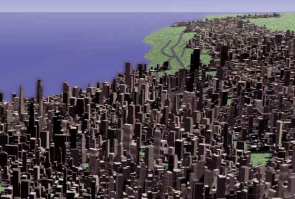
\includegraphics[width=0.6\columnwidth]{images/13_finalcity}
    \caption{L-System based city \label{fig:finalcity}}
    \end{center}
\end{figure}




\bibliographystyle{acmtog}
\nocite{*}
\bibliography{l_systems}


%\received{September 2z008}{March 2009}

\end{document}
